\documentclass[12pt,titlepage,landscape,a4paper]{article}

%QUELQUES PACKAGES PLUS OU MOINS UTILES
\special{landscape}
\usepackage[T1]{fontenc}
\usepackage[latin1]{inputenc}
\usepackage[english]{babel}
\usepackage{amsfonts, amsmath, amssymb, amsthm, stmaryrd}
\usepackage{aeguill}
\usepackage{graphics, graphicx}
\usepackage{xcolor}
\usepackage{geometry}
\usepackage{paralist}
\usepackage{multido,ifthen}
\usepackage{tikz}\usetikzlibrary{trees,shapes,arrows,matrix,calc,arrows.meta}
\usepackage{hyperref}
\usepackage{movie15}
\usepackage[abs]{overpic}
\usepackage{xargs}
\usepackage{extarrows}
\usepackage{shuffle}
\usepackage{multicol}
\usepackage{etoolbox}
\usepackage{dsfont}
\usepackage{pifont}
\usepackage{array, blkarray}
\usepackage{multicol, multirow}
\usepackage{ulem}
\usepackage{xifthen}

% ZONE DE TEXTE ET POLICE
\setlength{\topmargin}{-2.8cm}
\setlength{\textheight}{19cm}
\setlength{\oddsidemargin}{-1cm}
\setlength{\textwidth}{26.8cm}
\newcommand{\textenormal}{\fontsize{22}{28}\selectfont}
\newcommand{\textemoyen}{\fontsize{24}{27}\selectfont}
\newcommand{\textegrand}{\fontsize{55}{48}\selectfont}

% COMMANDE DE NOUVELLE PAGE
\newenvironment{slide}[1]
{
\newpage
\begin{center}
{\blue \textemoyen \uppercase{#1}}\\
\end{center}
\vspace{-1cm}
\rule{\textwidth}{0.5 pt}\\
\vspace{-.8cm}
}
{\vspace*{-3cm}}

% COMMANDE DE PARTIE
%\newcounter{partie}
%\setcounter{partie}{1}
%\newcommand{\thePartie}{Part \arabic{partie}}
\newcommand{\partie}[1]
{
\newpage
\vspace*{0pt plus 1 fill}
\begin{center}
%\thePartie \\[-.75cm]
\rule{.8\textwidth}{0.5 pt} \\[.5cm]
\fontsize{35}{35}\selectfont {\blue\uppercase{#1}} \\[-.35cm]
\rule{.8\textwidth}{0.5 pt} \\
\end{center}
\vspace*{0pt plus 1.2 fill}
%\addtocounter{partie}{1}
}

% COMMANDE D'EXPOSE
\newcommand{\expose}[2]
{
\newpage
\vspace*{0pt plus 1 fill}
\begin{center}
%\thePartie \\[-.75cm]
\rule{.8\textwidth}{0.5 pt} \\[.5cm]
\fontsize{35}{35}\selectfont {\red\uppercase{#1}} \\[-.35cm]
\rule{.8\textwidth}{0.5 pt} \\
\vspace{1cm}
\textemoyen #2
\end{center}
\vspace*{0pt plus 1.2 fill}
%\addtocounter{partie}{1}
}

% COMMANDE POUR LES BOITES
% centre
\newcommand{\cboite}[1]
{
\vspace*{.5cm}
\fcolorbox{blue}{grisclair}{
\begin{minipage}{.97\linewidth}
\vspace*{.3cm}
\begin{center} #1 \end{center}
\vspace*{-.1cm}
\end{minipage}
}
}
% alignement gauche
\newcommand{\gboite}[1]
{
\vspace*{.5cm}
\fcolorbox{blue}{grisclair}{
\begin{minipage}{.97\linewidth}
\vspace*{.3cm}
#1
\vspace{.3cm}
\end{minipage}
}
}

% AUTRES COMMANDES
% quelques couleurs manquantes
\newcommand{\orange}{\color{orange}} % couleur orange
\newcommand{\green}{\color{green}} % couleur verte
\newcommand{\violet}{\color{violet}} % couleur violet
\newcommand{\blue}{\color{blue}} % couleur bleu
\newcommand{\red}{\color{red}} % couleur rouge
\definecolor{violet}{rgb}{.5,.1,.9}
\definecolor{orange}{rgb}{.94,.57,0}
\definecolor{green}{rgb}{0.2,0.6,0.2}
\definecolor{grisclair}{gray}{1}
\definecolor{grisfonce}{gray}{.1}
\definecolor{bblue}{rgb}{.8,.8,1}
% maths
\newcommand{\set}[2]{\left\{ #1 \;\middle|\; #2 \right\}} % ensemble
\newcommand{\bigset}[2]{\big\{ #1 \;\big|\; #2 \big\}} % ensemble
\newcommand{\biggset}[2]{\bigg\{ #1 \;\bigg|\; #2 \bigg\}} % ensemble
\newcommand{\setangle}[2]{\left\langle #1 \;\middle|\; #2 \right\rangle} % ensemble
\newcommand{\dotprod}[2]{\left\langle\; #1 \;\middle|\; #2 \;\right\rangle} % produit scalaire
\newcommand{\ssm}{\smallsetminus} % small set minus
\newcommand{\symdif}{\triangle} % symmetric difference
\newcommand{\eqdef}{\mbox{\,\raisebox{0.3ex}{\normalsize\ensuremath{\mathrm:}}\ensuremath{=}\,}} % :=
\newcommand{\defeq}{\mbox{~\ensuremath{=}\raisebox{0.3ex}{\normalsize\ensuremath{\mathrm:}} }} % =:
\newcommand{\Fracfloor}[2]{\left\lfloor \frac{#1}{#2} \right\rfloor} % floor of a fraction
\newcommand{\one}{1\!\!1} % one bold
\DeclareMathOperator{\conv}{conv} % enveloppe convexe
\DeclareMathOperator{\cone}{cone} % cone engendre
\DeclareMathOperator{\vol}{vol} % volume
\newcommand{\C}{\mathbb{C}} % complexes
\newcommand{\R}{\mathbb{R}} % reels
\newcommand{\Z}{\mathbb{Z}} % entiers
\newcommand{\N}{\mathbb{N}} % naturels
\newcommand{\I}{\mathbb{I}} % set of integers
\newcommand{\K}{\mathbb{K}} % field
\newcommand{\fS}{\mathfrak{S}} % symmetric group
\newcommand{\cA}{\mathcal{A}} % algebra
\newcommand{\cF}{\mathcal{F}} % flip graph
\newcommand{\cN}{\mathcal{N}} % sorting network
\renewcommand{\b}[1]{\mathbf{#1}} % bold letters
\renewcommand{\c}[1]{\mathcal{#1}} % caligraphic letters
\newcommand{\f}[1]{\mathfrak{#1}} % frak letters
% autres
\setlength{\parindent}{0pt} % aucune indentation dans tout le document
\graphicspath{{figures/}} % les repertoires ou se trouvent les figures
\newcommand{\papier}[1]{\begin{flushright} {\violet \fontsize{15}{20}\selectfont #1} \end{flushright}} % citation papier
\newcommand{\theo}[2]{\gboite{{\blue \fontsize{18}{25}\selectfont #1.} #2}}
\newcommand{\HUGE}[1]{{\fontsize{35}{33}\selectfont #1}}
\newcommand{\esperluette}{ \\ --- \& --- \\ } % esperluette stylis�e nouvelle ligne
\DeclareRobustCommand{\verylongrightarrow}{\joinrel\relbar\joinrel\relbar\joinrel\relbar\joinrel\relbar\joinrel\relbar\joinrel\rightarrow}
\renewcommand{\emph}[1]{{\blue #1}}

% POLYTOPES
\newcommand{\Asso}{\mathsf{Asso}} % associahedron
\newcommandx{\Brick}[2][1=k, 2=n]{\mathsf{Brick}^{#1}(#2)} % brick polytope
\newcommand{\Perm}{\mathsf{Perm}} % permutahedron
\newcommand{\Para}{\mathsf{Para}} % parallelepiped
\newcommandx{\Zono}{\mathsf{Zono}} % zonotope
\newcommand{\Hyp}{\b{H}^=} % hyperplane
\newcommand{\HS}{\b{H}^\ge} % half-space
\newcommand{\HH}{\mathbb{H}} % hyperplane
\newcommand{\Cone}{\mathrm{C}} % cone
\newcommand{\polar}{^\diamond} % polar
\newcommand{\vertex}[1]{\b{a}(#1)} % vertex corresponding to a maximal signed nested set
\newcommand{\face}[1]{\b{f}(#1)} % face corresponding to a signed nested set
\newcommand{\braidFan}{\mathcal{B\!F}} % braid fan
\newcommand{\secPoly}{\Sigma\mathsf{Poly}} % secondary polytope
\newcommand{\secFan}{\Sigma\mathsf{Fan}} % secondary fan
\newcommand{\rhs}[2]{\omega(#1, #2)} % right hand side of zonotope

% LATTICES
\newcommand{\meet}{\wedge} % meet
\newcommand{\join}{\vee} % join
\newcommand{\bigMeet}{\bigwedge} % meet
\newcommand{\bigJoin}{\bigvee} % join
\newcommand{\closure}[1]{#1^{\mathrm{cl}}} % closure operator
\newcommand{\coclosure}[1]{#1^{\mathrm{cocl}}} % coclosure operator
\newcommand{\Bicl}[1]{\mathsf{Bic}(#1)} % biclosed sets
\newcommand{\projDown}{\pi_\downarrow} % down projection map
\newcommand{\projUp}{\pi^\uparrow} % up projection map
\newcommand{\JI}{\mathsf{JI}} % join-irreducible
\newcommand{\MI}{\mathsf{MI}} % meet-irreducible
\newcommand{\Cong}{\mathsf{Cong}} % congruence lattice
\newcommand{\con}{\mathrm{con}} % congruence contracting a cover relation
\newcommand{\ji}{\mathsf{ji}} % join irreducible
\newcommand{\mi}{\mathsf{mi}} % meet irreducible
\newcommand{\Pos}{\mathrm{Pos}} % poset of regions

% NONKISSING COMPLEX
\newcommand{\blossom}{^\text{\ding{96}}} % blossom
\renewcommand{\top}{\mathrm{top}} % top
\newcommand{\bottom}{\mathrm{bot}} % bottom
\newcommandx{\NKC}[1][1=\bar Q]{\mathcal{NK}(#1)} % non-kissing complex
\newcommandx{\RNKC}[1][1=\bar Q]{\mathcal{NK}(#1)} % non-kissing complex
\newcommandx{\NKL}[1][1=\bar Q]{\mathcal{L}_{\mathrm{nk}}(#1)} % non-kissing lattice
\newcommand{\distinguishedWalk}[2]{\mathsf{dw}(#1,#2)} % distinguished walk
\newcommand{\distinguishedArrows}[2]{\mathsf{da}(#1,#2)} % distinguished arrows
\newcommand{\distinguishedString}[2]{\mathsf{ds}(#1,#2)} % distinguished string
\newcommand{\distinguishedSign}[2]{\varepsilon(#1,#2)} % distinguished sign
\newcommand{\peaks}[1]{\mathsf{peaks}(#1)} % peaks
\newcommand{\deeps}[1]{\mathsf{deeps}(#1)} % deeps
\newcommand{\kn}{\kappa} % kissing number
\newcommand{\KN}{\textsc{kn}} % Kissing Number
\newcommand{\gvector}{\b{g}} % g-vector
\newcommand{\gvectors}{\b{g}} % g-vectors
\newcommand{\gvectorFan}{\mathcal{F}^\b{g}} % g-vector fan
\newcommand{\cvector}{\b{c}} % c-vector
\newcommand{\cvectors}{\b{c}} % c-vectors
\newcommand{\allcvectors}[1]{\b{C}(#1)} % all c-vectors with respect to the initial cluster #1
\newcommand{\point}{\mathbf{p}} % vertex of the #1-associahedron corresponding to the cluster #2

%%%%%%%%%%%%%%%%%%%%%%%%%%%%%%%%%%%%%%%%%%%%%%%%

\newcommand{\titre}{More friends for the associahedron}
\newcommand{\auteur}{Vincent Pilaud}

%%%%%%%%%%%%%%%%%%%%%%%%%%%%%%%%%%%%%%%%%%%%%%%%

\begin{document}

\fontshape{sf}\fontsize{22}{28}\selectfont % police par defaut
\sf
\pagestyle{empty} % bas de page par defaut

%%%%%%%%%

\begin{flushright}
\vspace*{.3cm}

{\blue \fontsize{53}{50}\selectfont

NON-KISSING \\ COMPLEXES \\
FOR GENTLE \\ ALGEBRAS

}

\vspace{1.1cm}
\HUGE{Y. PALU} \\
Univ. Amiens

\vspace{1cm}
\HUGE{V. PILAUD} \\
CNRS \& LIX, \\ \'Ecole Poytechnique

\vspace{1cm}
\HUGE{P.-G. PLAMONDON} \\
Univ. Orsay

\end{flushright}

\vspace*{-18.5cm}%\hspace*{1cm}
\hspace*{-1.5cm}
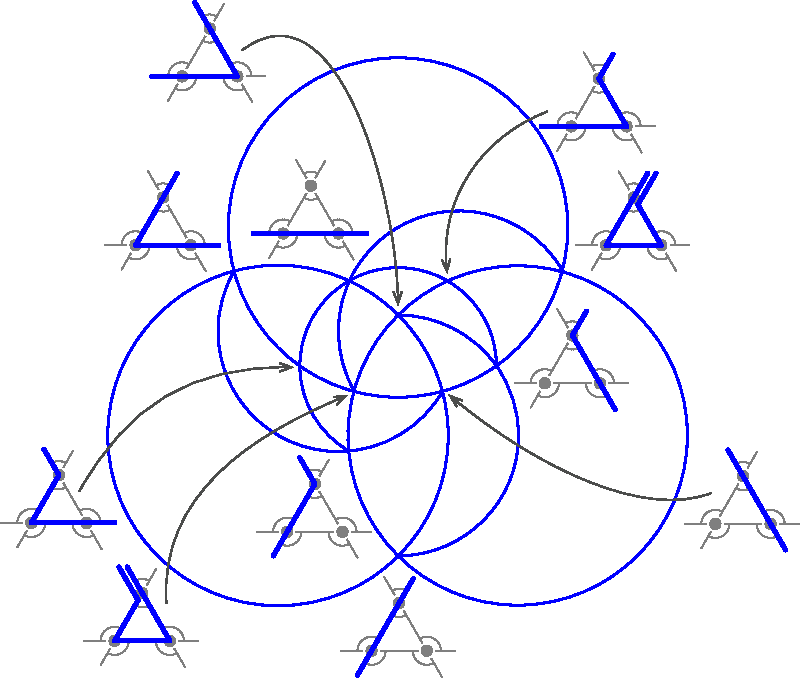
\includegraphics[scale=1.43]{title}
\vspace*{-3cm}

%%%%%%%%%

%\expose{IV. NON-KISSING COMPLEXES \\ AND GENTLE ASSOCIAHEDRA}{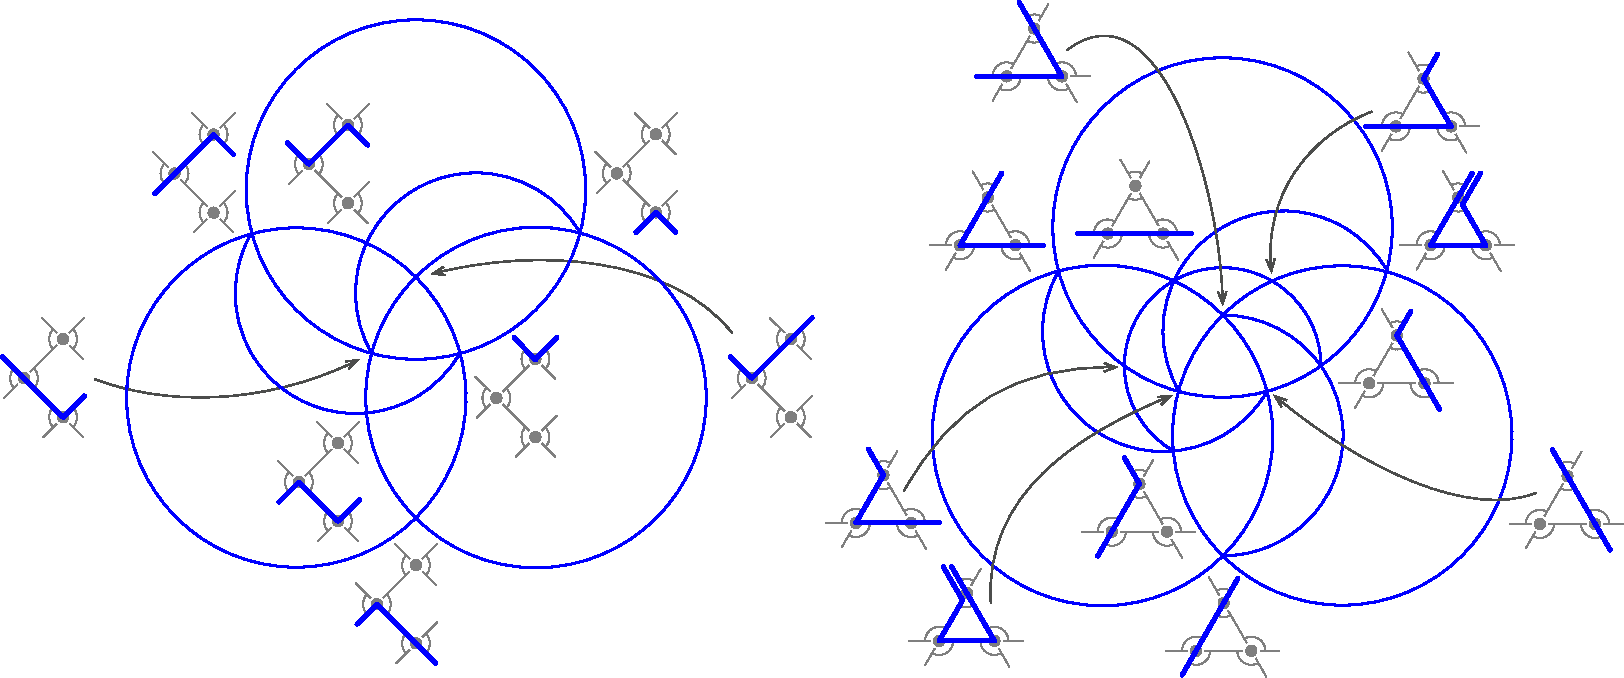
\includegraphics[scale=.95]{justFans}}
%
%\vspace*{-.2cm}
%\papier{\textemoyen Palu--P.--Plamondon, \textit{Non-kissing complexes and $\tau$-tilting for gentle alg.}~('17$^+$)
%\vspace*{-.5cm}
%}

%%%%%%%%%

\partie{Non-kissing complex}

\vspace*{-1.5cm}
\papier{\textemoyen
	Petersen--Pylyavskyy--Speyer, \textit{A non-crossing standard monomial theory} ('10) \\
	Santos--Stump-Welker, \textit{Non-crossing sets and the Grassmann-assoc.} ('17) \\
	McConville, \textit{Lattice structures of grid Tamari orders} ('17) \\
	Garver--McConville, \textit{Enumerative properties of grid-associahedra} ('17$^+$) \\
	Palu--P.--Plamondon, \textit{Non-kissing complexes and $\tau$-tilting for gentle alg.}~('17$^+$) \\
	Br\"ustle--Douville--Mousavand--Thomas--Y\i{}ld\i{}r\i{}m, \textit{On the combinatorics of gentle algebras} ('17$^+$) \\
}

%%%%%%%%%

\begin{slide}{Gentle quivers and strings}

\hspace{-1cm}
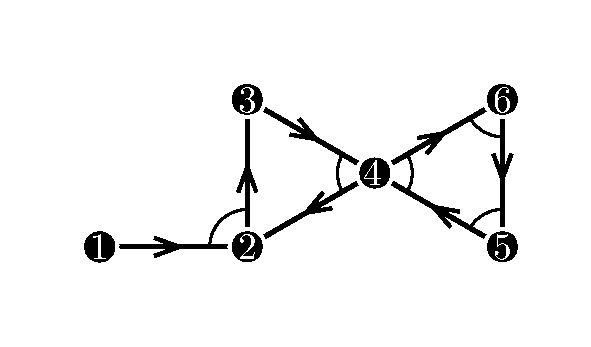
\includegraphics[scale=1.3]{exmQuiver}

\vspace{-7cm}
\hspace{12cm}
\begin{minipage}{14cm}
\emph{gentle quiver} $\bar Q$ =
\begin{compactitem}
\item \emph{quiver}~$Q$ = oriented graph $(Q_0, Q_1, s, t)$ % \\ (loops and multiple edges allowed)
\item \emph{relations}~$I$ = forbid certain paths
\end{compactitem}
where
\begin{compactitem}
\item forbidden paths all of length~$2$ \\[-1.3cm]
\item locally at each vertex, subgraph of \raisebox{-.9cm}{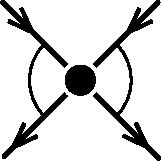
\includegraphics[scale=.8]{localGentle}}
\end{compactitem}
\end{minipage}

\end{slide}

%%%%%%%%%

\begin{slide}{Gentle quivers and strings}

\hspace{-1cm}
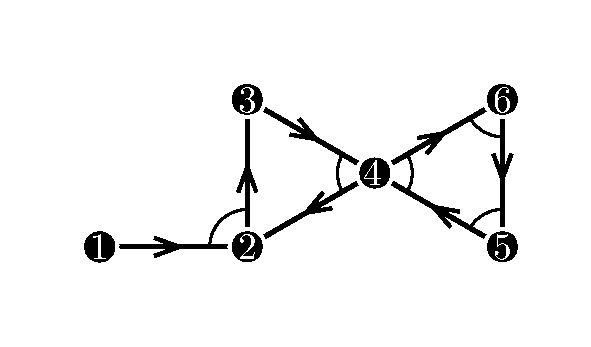
\includegraphics[scale=1.3]{exmQuiver}

\vspace{-7cm}
\hspace{12cm}
\begin{minipage}{14cm}
\emph{gentle quiver} $\bar Q$ =
\begin{compactitem}
\item \emph{quiver}~$Q$ = oriented graph $(Q_0, Q_1, s, t)$ % \\ (loops and multiple edges allowed)
\item \emph{relations}~$I$ = forbid certain paths
\end{compactitem}
where
\begin{compactitem}
\item forbidden paths all of length~$2$ \\[-1.3cm]
\item locally at each vertex, subgraph of \raisebox{-.9cm}{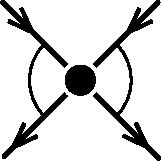
\includegraphics[scale=.8]{localGentle}}
\end{compactitem}
\end{minipage}

\vspace{1cm}

\hspace{-1cm}
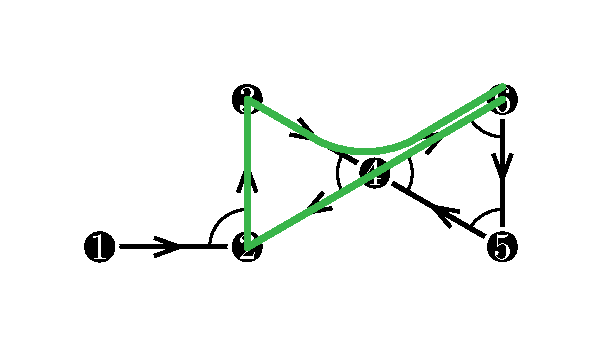
\includegraphics[scale=1.3]{exmString}

\vspace{-6cm}
\hspace{12cm}
\begin{minipage}{15cm}
\emph{string} $\sigma$ = 
\mbox{$\alpha_1^{\varepsilon_1} \dots \alpha_\ell^{\varepsilon_\ell}$ with $\alpha_k \in Q_1$, $\varepsilon_k \in \{-1,1\}$} \\
such that
\begin{compactitem}
\item $t(\alpha_k^{\varepsilon_k}) = s(\alpha_{k+1}^{\varepsilon_{k+1}})$
\item contains no factor~$\pi$ or~$\pi^{-1}$ for any path~$\pi \in I$
\item \mbox{contains no~$\alpha\alpha^{-1}$ or~$\alpha^{-1}\alpha$ for any arrow~$\alpha \in Q_1$}
\end{compactitem}
\end{minipage}

\end{slide}

%%%%%%%%%

\begin{slide}{Blossoming quivers and walks}

\hspace{-1cm}
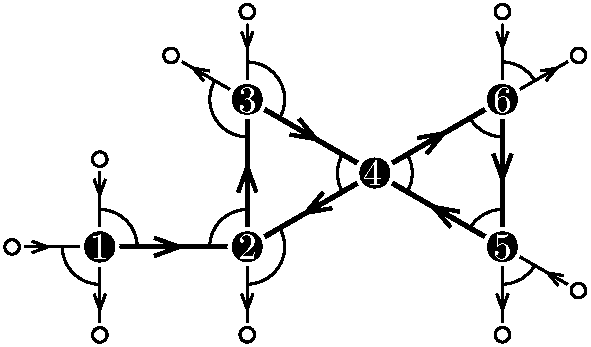
\includegraphics[scale=1.3]{exmBlossomingQuiver}

\vspace{-5cm}
\hspace{12.5cm}
\begin{minipage}{14.5cm}
\emph{blossoming quiver} $\bar Q\blossom$ = \\[-.5cm]
add blossoms to complete each vertex to \raisebox{-.9cm}{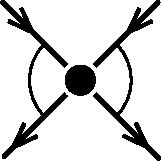
\includegraphics[scale=.8]{localGentle}}
\end{minipage}

\end{slide}

%%%%%%%%%

\begin{slide}{Blossoming quivers and walks}

\hspace{-1cm}
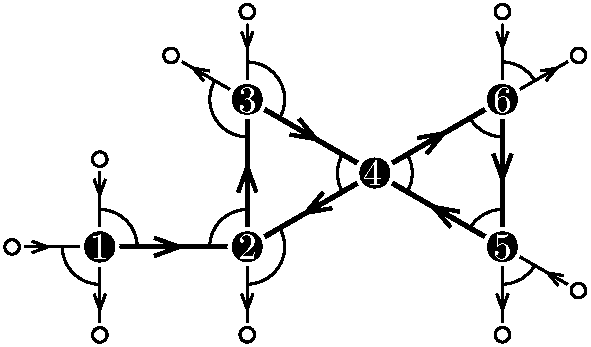
\includegraphics[scale=1.3]{exmBlossomingQuiver}

\vspace{-5cm}
\hspace{12.5cm}
\begin{minipage}{14.5cm}
\emph{blossoming quiver} $\bar Q\blossom$ = \\[-.5cm]
add blossoms to complete each vertex to \raisebox{-.9cm}{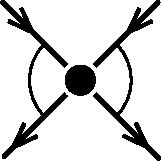
\includegraphics[scale=.8]{localGentle}}
\end{minipage}

\vspace{4cm}

\hspace{-1cm}
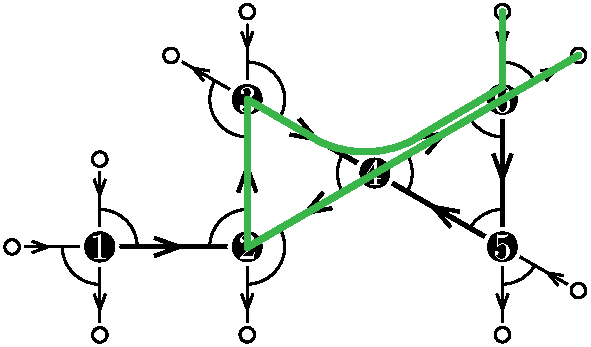
\includegraphics[scale=1.3]{exmWalk}

\vspace{-6cm}
\hspace{12cm}
\begin{minipage}{13cm}
\emph{walk} $\omega$ = 
\begin{tabular}[t]{l}
maximal string in $\bar Q\blossom$ \\
from blossoms to blossoms
\end{tabular}
\end{minipage}

\end{slide}

%%%%%%%%%

\begin{slide}{Kissing or crossing}

\vspace{.5cm}
%Two walks~$\omega, \omega'$ with a common substring can either:\\[.5cm]
\centerline{KISS \hspace{6cm} or \hspace{5.5cm} CROSS}
\vspace{-1.3cm}
\centerline{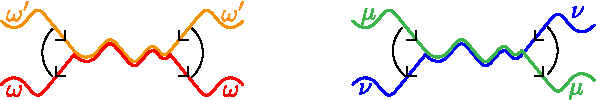
\includegraphics[scale=2.5]{kissingCrossing}}

\vspace{1.5cm}
\centerline{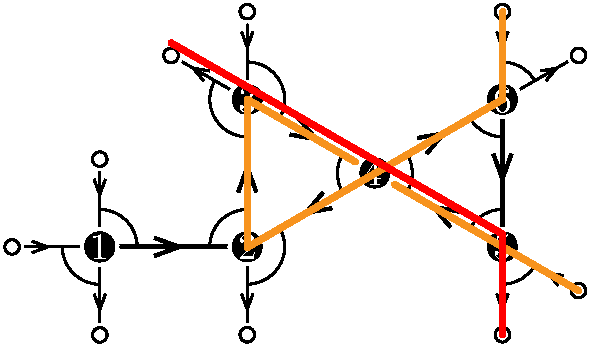
\includegraphics[scale=1.3]{exmKissing1}\qquad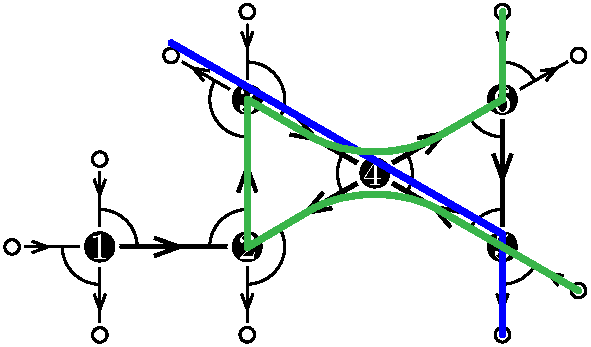
\includegraphics[scale=1.3]{exmNonKissing1}}

\end{slide}

%%%%%%%%%

\begin{slide}{Non-kissing complex}

\vspace{.5cm}
%Two walks~$\omega, \omega'$ with a common substring can either:\\[.5cm]
\centerline{KISS \hspace{6cm} \phantom{or \hspace{5.5cm} CROSS}}
\vspace{-1.3cm}
\centerline{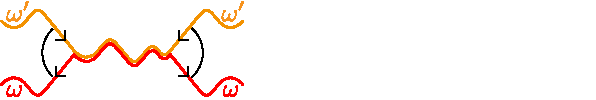
\includegraphics[scale=2.5]{kissing}}

\vspace{.5cm}
[reduced] \emph{non-kissing complex} $\NKC$ = % \\ simplicial complex with
\begin{compactitem}
\item vertices = [bending] walks in $\bar Q\blossom$ \\ (that are not self-kissing)
\item faces = collections of pairwise \\ non-kissing [bending] walks in $\bar Q\blossom$
\end{compactitem}

\vspace{.3cm}
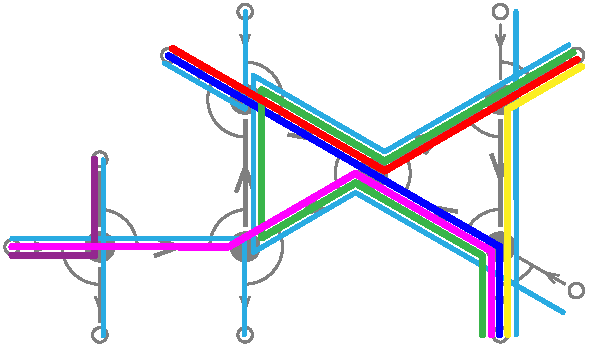
\includegraphics[scale=1.3]{exmFacet}

\vspace{-17cm}\hspace{13cm}
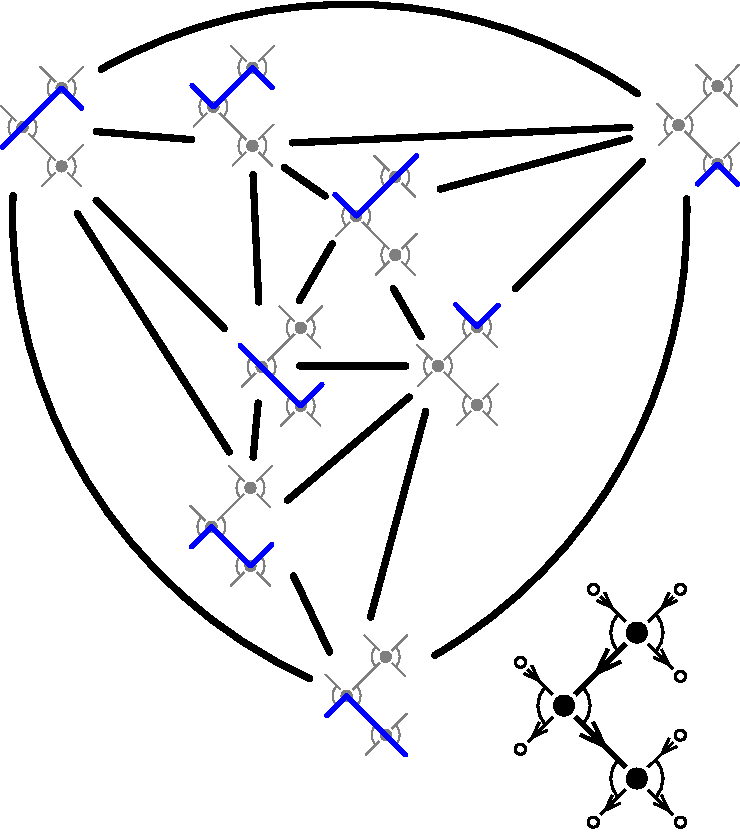
\includegraphics[scale=1.1]{exmNKC}

\end{slide}

%%%%%%%%%

\begin{slide}{Simplicial associahedra are non-kissing complexes}

\vspace{.5cm}
[reduced] \emph{simplicial associahedron} = simplicial complex with
\begin{compactitem}
\item vertices = [internal] diagonals of an $(n+3)$-gon
\item faces = collections of pairwise non-crossing [internal] diagonals of the $(n+3)$-gon
\end{compactitem}

\vspace{1.5cm}
\centerline{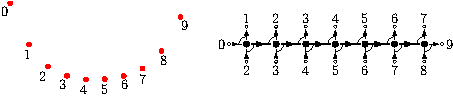
\includegraphics[scale=3.5]{exmBijectionAssociahedron1}}

\end{slide}

%%%%%%%%%

\begin{slide}{Simplicial associahedra are non-kissing complexes}

\vspace{.5cm}
[reduced] \emph{simplicial associahedron} = simplicial complex with
\begin{compactitem}
\item vertices = [internal] diagonals of an $(n+3)$-gon
\item faces = collections of pairwise non-crossing [internal] diagonals of the $(n+3)$-gon
\end{compactitem}

\vspace{1.5cm}
\centerline{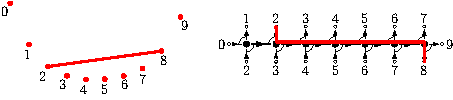
\includegraphics[scale=3.5]{exmBijectionAssociahedron2}}

\vspace{1cm}
\centerline{
\begin{tabular}{c@{\hspace{2cm}$\longleftrightarrow$\hspace{2cm}}c}
\hspace{3cm} diagonal \hspace{3cm} &  \hspace{3cm} walk \hspace{3cm} \\[2cm]
\end{tabular}
}

\end{slide}

%%%%%%%%%

\begin{slide}{Simplicial associahedra are non-kissing complexes}

\vspace{.5cm}
[reduced] \emph{simplicial associahedron} = simplicial complex with
\begin{compactitem}
\item vertices = [internal] diagonals of an $(n+3)$-gon
\item faces = collections of pairwise non-crossing [internal] diagonals of the $(n+3)$-gon
\end{compactitem}

\vspace{1.5cm}
\centerline{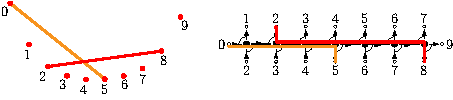
\includegraphics[scale=3.5]{exmBijectionAssociahedron3}}

\vspace{1cm}
\centerline{
\begin{tabular}{c@{\hspace{2cm}$\longleftrightarrow$\hspace{2cm}}c}
\hspace{3cm} diagonal \hspace{3cm} &  \hspace{3cm} walk \hspace{3cm} \\
crossing & kissing
\end{tabular}
}

\end{slide}

%%%%%%%%%

\begin{slide}{Simplicial associahedra are non-kissing complexes}

\vspace{.5cm}
[reduced] \emph{simplicial associahedron} = simplicial complex with
\begin{compactitem}
\item vertices = [internal] diagonals of an $(n+3)$-gon
\item faces = collections of pairwise non-crossing [internal] diagonals of the $(n+3)$-gon
\end{compactitem}

\vspace{1.5cm}
\centerline{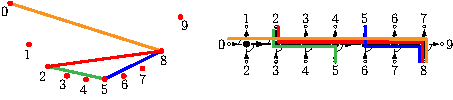
\includegraphics[scale=3.5]{exmBijectionAssociahedron4}}

\vspace{1cm}
\centerline{
\begin{tabular}{c@{\hspace{2cm}$\longleftrightarrow$\hspace{2cm}}c}
\hspace{3cm} diagonal \hspace{3cm} &  \hspace{3cm} walk \hspace{3cm} \\
crossing & kissing \\
dissection & non-kissing face
\end{tabular}
}

\end{slide}

%%%%%%%%%

\begin{slide}{Simplicial associahedra are non-kissing complexes}

\vspace{.5cm}
[reduced] \emph{simplicial associahedron} = simplicial complex with
\begin{compactitem}
\item vertices = [internal] diagonals of an $(n+3)$-gon
\item faces = collections of pairwise non-crossing [internal] diagonals of the $(n+3)$-gon
\end{compactitem}

\vspace{1.5cm}
\centerline{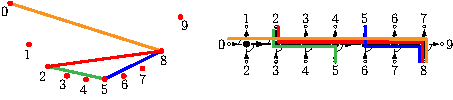
\includegraphics[scale=3.5]{exmBijectionAssociahedron4}}

\vspace{1cm}
\centerline{
\begin{tabular}{c@{\hspace{2cm}$\longleftrightarrow$\hspace{2cm}}c}
\hspace{3cm} diagonal \hspace{3cm} &  \hspace{3cm} walk \hspace{3cm} \\
crossing & kissing \\
dissection & non-kissing face \\
simplicial associahedron & non-kissing complex
\end{tabular}
}

\vspace{.3cm}
\papier{McConville, \textit{Lattice structures of grid Tamari orders} ('17)}


\end{slide}

%%%%%%%%%%
%
%\begin{slide}{Simplicial associahedra are non-kissing complexes}
%
%\vspace{.5cm}
%[reduced] \emph{simplicial associahedron} = simplicial complex with
%\begin{compactitem}
%\item vertices = [internal] diagonals of an $(n+3)$-gon
%\item faces = collections of pairwise non-crossing [internal] diagonals of the $(n+3)$-gon
%\end{compactitem}
%
%\vspace{1.5cm}
%\centerline{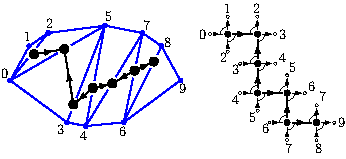
\includegraphics[scale=3.5]{exmBijectionAssociahedron5}}
%
%\vspace{1.2cm}
%\papier{McConville, \textit{Lattice structures of grid Tamari orders} ('17)}
%
%\end{slide}
%
%%%%%%%%%%

\begin{slide}{Two more families of non-kissing complexes}

\vspace{.3cm}
\centerline{
\begin{tabular}{c@{\hspace{3cm}}c}
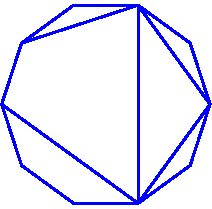
\includegraphics[scale=2]{exmDissection1} & 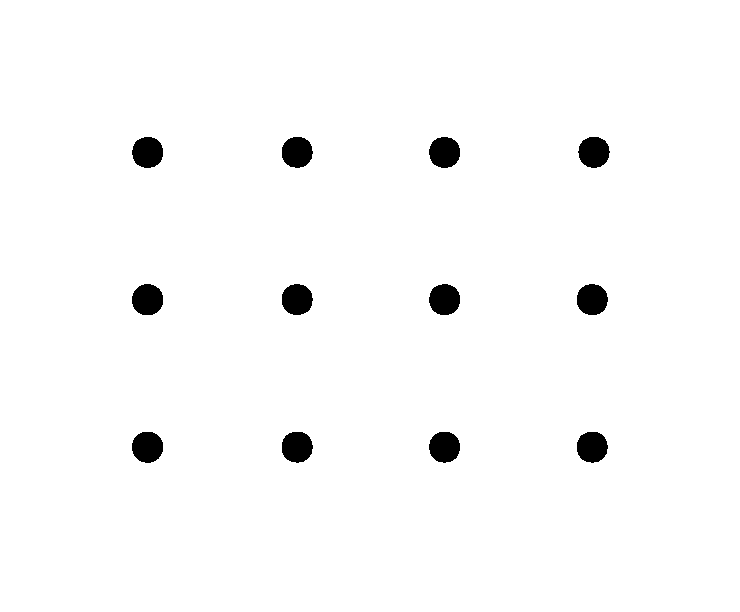
\includegraphics[scale=.7]{exmGrid1} \\[.2cm]
dissection & subset of $\Z^2$
\end{tabular}
}

\end{slide}

%%%%%%%%%

\begin{slide}{Two more families of non-kissing complexes}

\vspace{.3cm}
\centerline{
\begin{tabular}{c@{\hspace{3cm}}c}
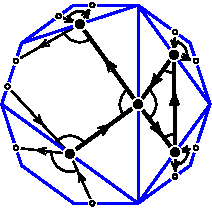
\includegraphics[scale=2]{exmDissection2} & 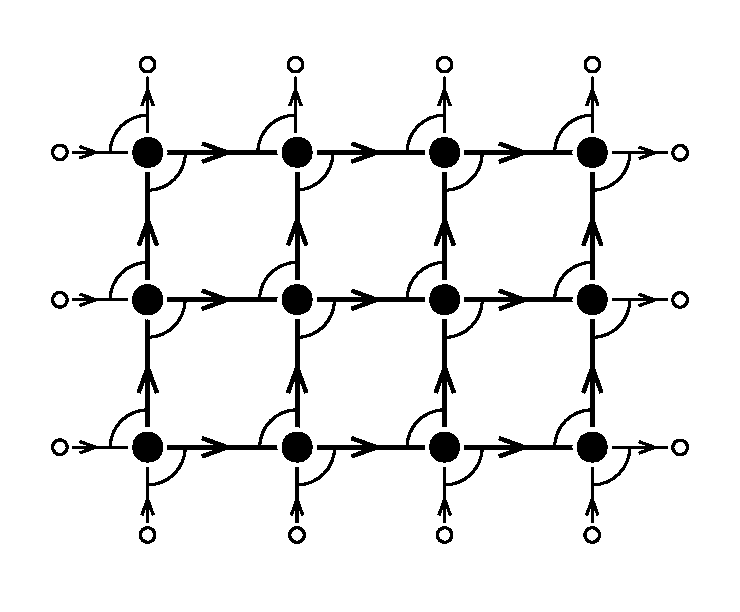
\includegraphics[scale=.7]{exmGrid2} \\[.2cm]
dissection & subset of $\Z^2$
\end{tabular}
}

\end{slide}

%%%%%%%%%%
%
%\begin{slide}{Two more families of non-kissing complexes}
%
%\vspace{.3cm}
%\centerline{
%\begin{tabular}{c@{\hspace{3cm}}c}
%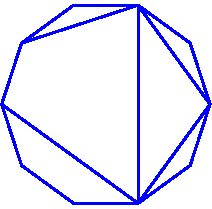
\includegraphics[scale=2]{exmDissection3t} & 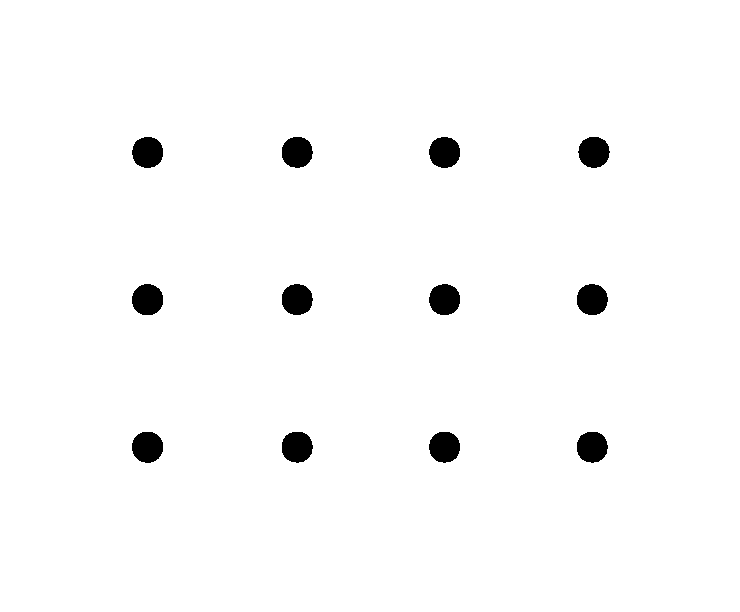
\includegraphics[scale=.7]{exmGrid3t} \\[.2cm]
%dissection & subset of $\Z^2$ \\[.5cm]
%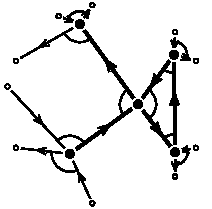
\includegraphics[scale=2]{exmDissection3b} & 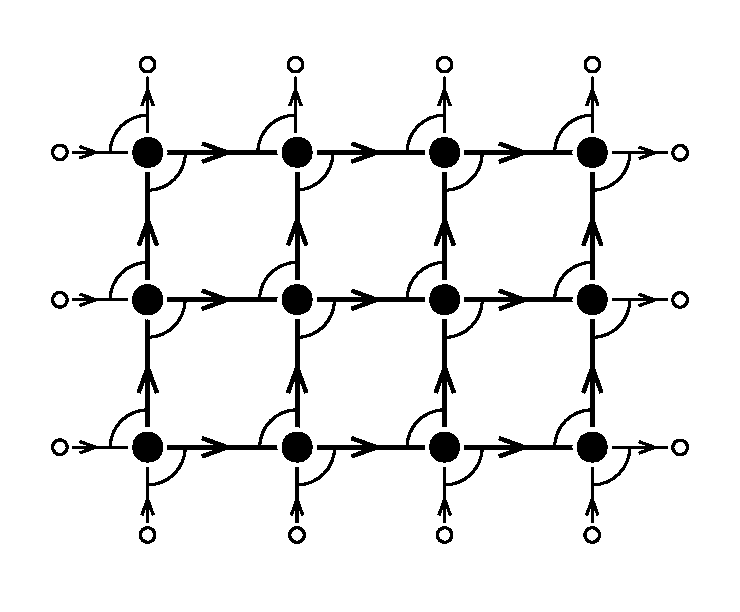
\includegraphics[scale=.7]{exmGrid3b} \\[.2cm]
%dissection quiver & grid quiver
%\end{tabular}
%}
%
%\end{slide}
%
%%%%%%%%%%
%
%\begin{slide}{Two more families of non-kissing complexes}
%
%\vspace{.3cm}
%\centerline{
%\begin{tabular}{c@{\hspace{3cm}}c}
%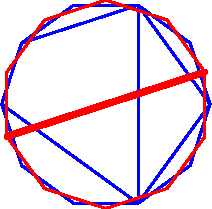
\includegraphics[scale=2]{exmDissection4t} & 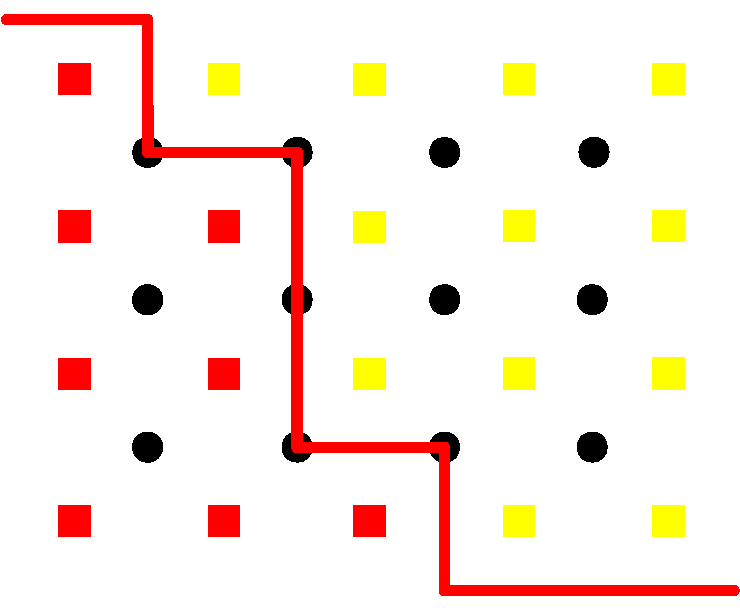
\includegraphics[scale=.7]{exmGrid4t} \\[.2cm]
%accordion & $2457$ subset of $[n+m]$ \\[.5cm]
%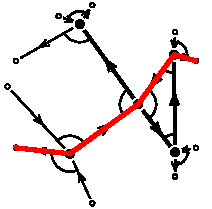
\includegraphics[scale=2]{exmDissection4b} & 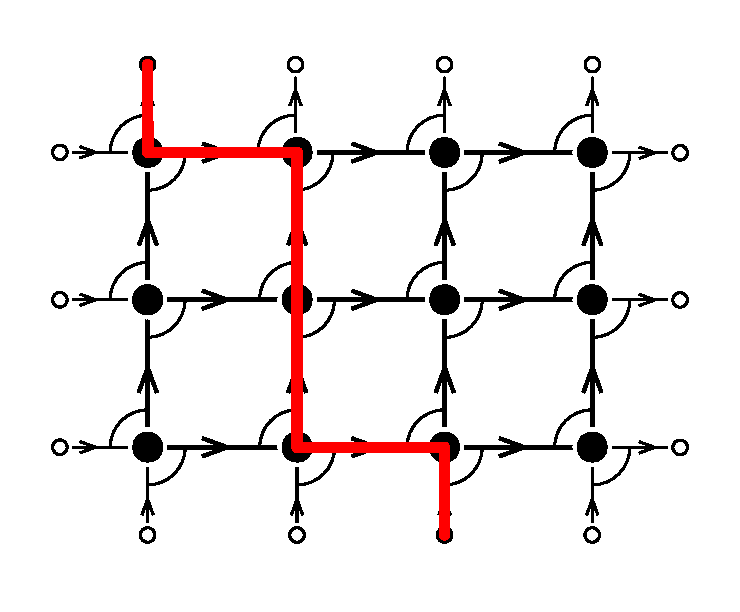
\includegraphics[scale=.7]{exmGrid4b} \\[.2cm]
%walk & walk
%\end{tabular}
%}
%
%\end{slide}
%
%%%%%%%%%%
%
%\begin{slide}{Two more families of non-kissing complexes}
%
%\vspace{.3cm}
%\centerline{
%\begin{tabular}{c@{\hspace{3cm}}c}
%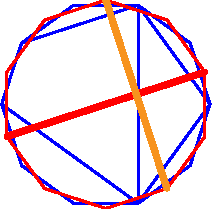
\includegraphics[scale=2]{exmDissection5t} & 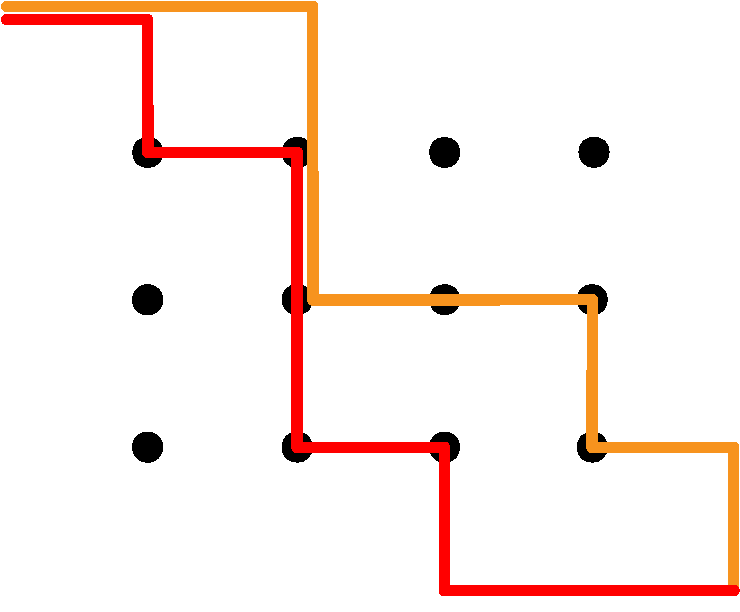
\includegraphics[scale=.7]{exmGrid5t} \\[.2cm]
%crossing accordions & crossing subsets of $[n+m]$ \\[.5cm]
%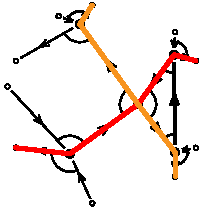
\includegraphics[scale=2]{exmDissection5b} & 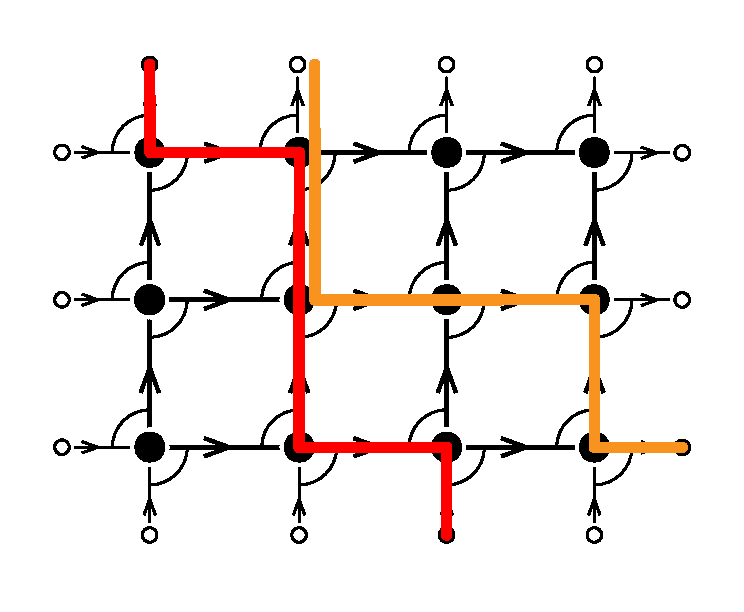
\includegraphics[scale=.7]{exmGrid5b} \\[.2cm]
%kissing walks & kissing walks
%\end{tabular}
%}
%
%\end{slide}

%%%%%%%%%

\begin{slide}{Two more families of non-kissing complexes}

\vspace{.3cm}
\centerline{
\begin{tabular}{c@{\hspace{3cm}}c}
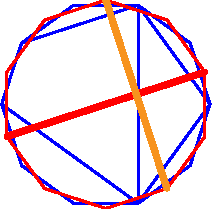
\includegraphics[scale=2]{exmDissection5t} & 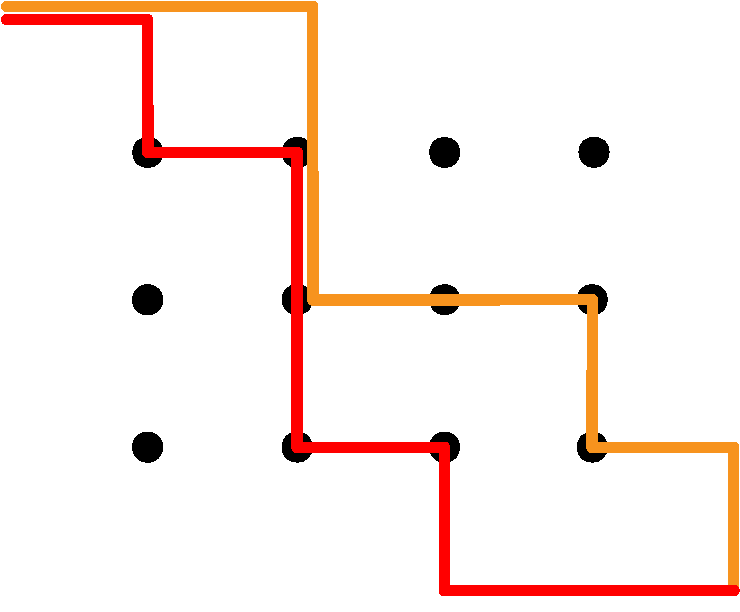
\includegraphics[scale=.7]{exmGrid5t} \\[.2cm]
accordion complex & grid Tamari complex \\[.5cm]
\end{tabular}
}

\vspace{.2cm}
\papier{

\flushleft 
Baryshnikov, \textit{On Stokes sets} ('01) \\
Chapoton, \textit{Stokes posets and serpent nests} ('16) \\
Garver--McConville, \textit{Oriented flip graphs and non-crossing tree partitions} ('18) \\[1cm]
\flushright
	Petersen--Pylyavskyy--Speyer, \textit{A non-crossing standard monomial theory} ('10) \\
	Santos--Stump--Welker, \textit{Non-crossing sets and the Grassmann-assoc.} ('17) \\
	McConville, \textit{Lattice structures of grid Tamari orders} ('17) \\
	Garver--McConville, \textit{Enumerative properties of grid-associahedra} ('17$^+$) \\
}

\vspace{.3cm}
The associahedron is an example of both...

\end{slide}

%%%%%%%%%

\begin{slide}{Overview of the talk}

\emph{non-kissing complex} $\NKC$ = % \\ simplicial complex with
\begin{compactitem}
\item vertices = walks in $\bar Q\blossom$ (that are not self-kissing)
\item faces = collections of pairwise non-kissing walks in $\bar Q\blossom$
\end{compactitem}

\vspace{-3cm}
\hspace{18cm}
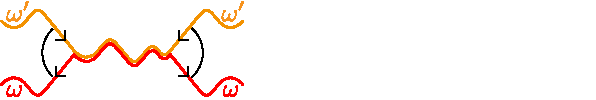
\includegraphics[scale=2]{kissing}

\vspace{-.3cm}
\emph{... generalizing the associahedron}

\vspace{.9cm}
\centerline{
\begin{tabular}{ccc}
Flip graph &
Associahedron &
Tamari lattice \\[.3cm]
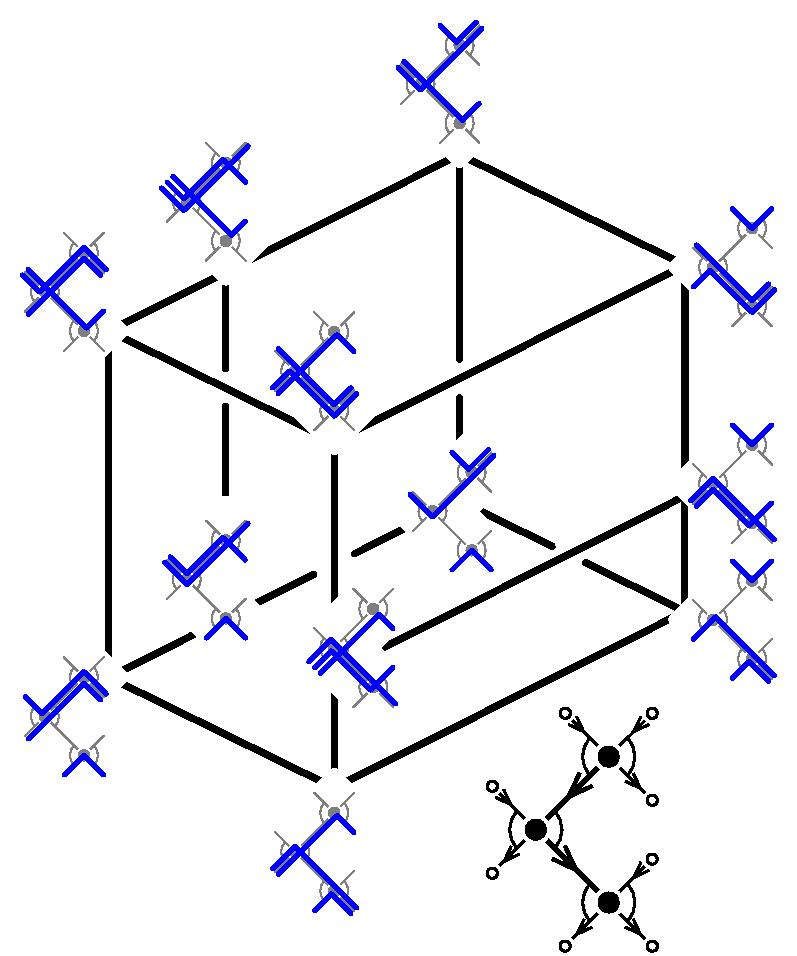
\includegraphics[scale=.7]{exmFlipGraph} &
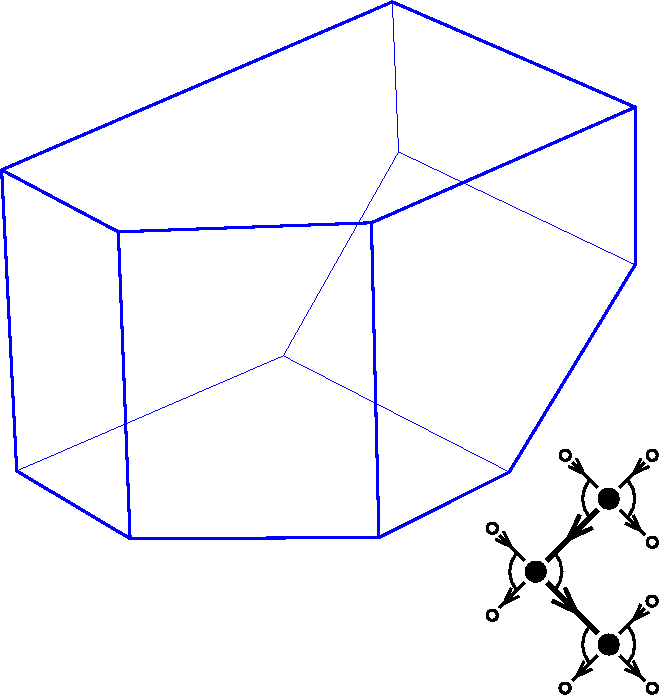
\includegraphics[scale=.7]{exmAssociahedron} & 
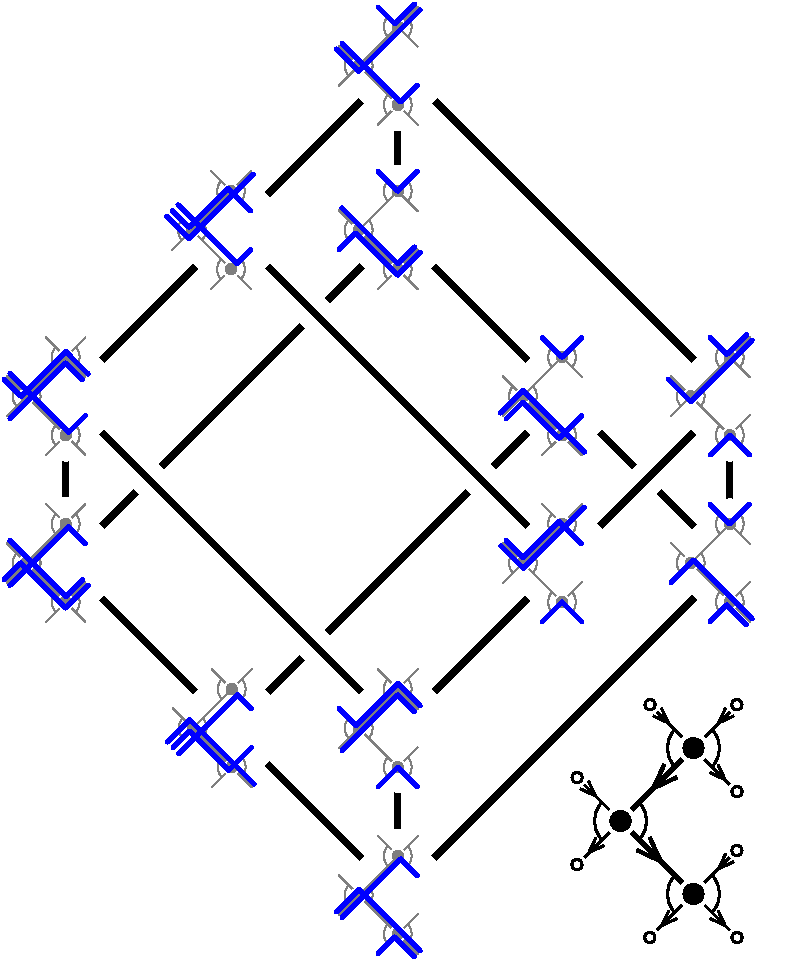
\includegraphics[scale=.7]{exmLattice} \\
\end{tabular}
}

\end{slide}

%%%%%%%%%

\partie{Distinguished arrows and flips}

\vspace*{-1.5cm}
\papier{\textemoyen
	McConville, \textit{Lattice structures of grid Tamari orders} ('17) \\
	Palu--P.--Plamondon, \textit{Non-kissing complexes and $\tau$-tilting for gentle alg.}~('17$^+$) \\
}

%%%%%%%%%

\begin{slide}{Distinguished walks, arrows and strings}

\vspace{1cm}
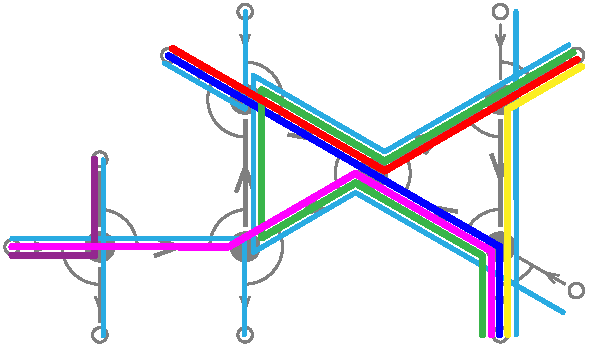
\includegraphics[scale=1.3]{exmFacet}

\vspace{-8.2cm}
\hspace{14cm}
\begin{minipage}{13cm}
$F$ face of $\NKC$ \\[.3cm]
\end{minipage}

\end{slide}

%%%%%%%%%

\begin{slide}{Distinguished walks, arrows and strings}

\vspace{1cm}
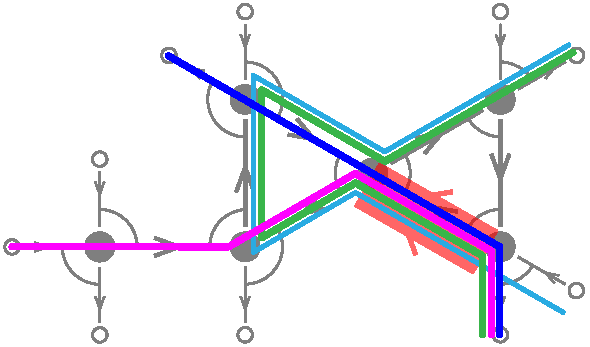
\includegraphics[scale=1.3]{exmCountercurrentOrder}

\vspace{-8.2cm}
\hspace{14cm}
\begin{minipage}{13cm}
$F$ face of $\NKC$ \\[.3cm]
${\red \alpha} \in Q_1$ \\
$F_{\red \alpha} = \set{\omega \in F}{{\red \alpha} \in \omega}$
\end{minipage}

\end{slide}

%%%%%%%%%

\begin{slide}{Distinguished walks, arrows and strings}

\vspace{1cm}
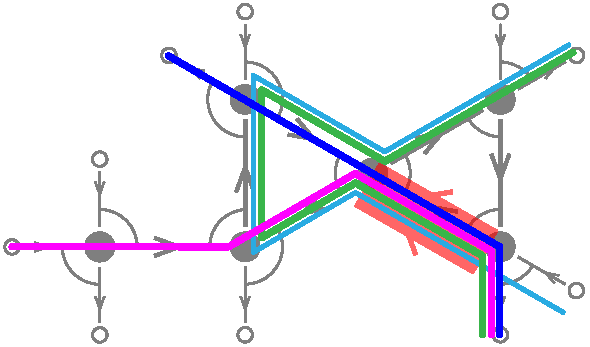
\includegraphics[scale=1.3]{exmCountercurrentOrder}

\vspace{-8.2cm}
\hspace{14cm}
\begin{minipage}{13cm}
$F$ face of $\NKC$ \\[.3cm]
${\red \alpha} \in Q_1$ \\
$F_{\red \alpha} = \set{\omega \in F}{{\red \alpha} \in \omega}$ \\[.3cm]
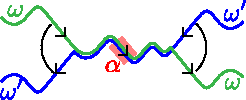
\includegraphics[scale=2.5]{crossing} \\[.1cm]
${\green \omega} \prec_{\red \alpha} {\blue \omega'}$ \emph{countercurrent order} at~${\red \alpha}$
\end{minipage}

\end{slide}

%%%%%%%%%

\begin{slide}{Distinguished walks, arrows and strings}

\vspace{1cm}
\includegraphics[scale=1.3]{exmDistinguishedArrow}

\vspace{-8.2cm}
\hspace{14cm}
\begin{minipage}{13cm}
$F$ face of $\NKC$ \\[.3cm]
${\red \alpha} \in Q_1$ \\
$F_{\red \alpha} = \set{\omega \in F}{{\red \alpha} \in \omega}$ \\[.3cm]
\includegraphics[scale=2.5]{crossing} \\[.1cm]
${\green \omega} \prec_\alpha {\blue \omega'}$ \emph{countercurrent order} at~${\red \alpha}$
\end{minipage}

\vspace{1cm}
\emph{distinguished walk} at~$\red \alpha$ in~$F$ = $\distinguishedWalk{{\red \alpha}}{F} = \max_{\prec_{\red \alpha}} F_{\red \alpha}$ \\
\emph{distinguished arrows} of~$\blue \omega$ in~$F$ = $\distinguishedArrows{{\blue \omega}}{F} = \set{{\red \alpha} \in Q_1}{{\blue \omega} = \distinguishedWalk{{\red \alpha}}{F}}$

\end{slide}

%%%%%%%%%

\begin{slide}{Distinguished walks, arrows and strings}

\vspace{1cm}
\includegraphics[scale=1.3]{exmDistinguished}

\vspace{-8.2cm}
\hspace{14cm}
\begin{minipage}{13cm}
$F$ face of $\NKC$ \\[.3cm]
${\red \alpha} \in Q_1$ \\
$F_{\red \alpha} = \set{\omega \in F}{{\red \alpha} \in \omega}$ \\[.3cm]
\includegraphics[scale=2.5]{crossing} \\[.1cm]
${\green \omega} \prec_\alpha {\blue \omega'}$ \emph{countercurrent order} at~${\red \alpha}$
\end{minipage}

\vspace{1cm}
\emph{distinguished walk} at~$\red \alpha$ in~$F$ = $\distinguishedWalk{{\red \alpha}}{F} = \max_{\prec_{\red \alpha}} F_{\red \alpha}$ \\
\emph{distinguished arrows} of~$\blue \omega$ in~$F$ = $\distinguishedArrows{{\blue \omega}}{F} = \set{{\red \alpha} \in Q_1}{{\blue \omega} = \distinguishedWalk{{\red \alpha}}{F}}$

\theo{PROP}{For any facet $F \in \NKC$, 
\begin{compactitem}
\item each bending walk of~$F$ contains $2$ distinguished arrows in~$F$ pointing opposite,
\item each straight walk of~$F$ contains $1$ distinguished arrows in~$F$ pointing as the walk.
\end{compactitem}
}

\end{slide}

%%%%%%%%%

\begin{slide}{Distinguished walks, arrows and strings}

\vspace{1cm}
\includegraphics[scale=1.3]{exmDistinguished}

\vspace{-8.2cm}
\hspace{14cm}
\begin{minipage}{13cm}
$F$ face of $\NKC$ \\[.3cm]
${\red \alpha} \in Q_1$ \\
$F_{\red \alpha} = \set{\omega \in F}{{\red \alpha} \in \omega}$ \\[.3cm]
\includegraphics[scale=2.5]{crossing} \\[.1cm]
${\green \omega} \prec_\alpha {\blue \omega'}$ \emph{countercurrent order} at~${\red \alpha}$
\end{minipage}

\vspace{1cm}
\emph{distinguished walk} at~$\red \alpha$ in~$F$ = $\distinguishedWalk{{\red \alpha}}{F} = \max_{\prec_{\red \alpha}} F_{\red \alpha}$ \\
\emph{distinguished arrows} of~$\blue \omega$ in~$F$ = $\distinguishedArrows{{\blue \omega}}{F} = \set{{\red \alpha} \in Q_1}{{\blue \omega} = \distinguishedWalk{{\red \alpha}}{F}}$

\theo{PROP}{For any facet $F \in \NKC$, 
\begin{compactitem}
\item each bending walk of~$F$ contains $2$ distinguished arrows in~$F$ pointing opposite,
\item each straight walk of~$F$ contains $1$ distinguished arrows in~$F$ pointing as the walk.
\end{compactitem}
}

\theo{CORO}{$\NKC$ is pure of dimension $|Q_0|$.}
\end{slide}

%%%%%%%%%

\begin{slide}{Flips}

\vspace{1cm}
\includegraphics[scale=1.3]{exmFlip0}

\vspace{1cm}
$F$ facet of $\NKC$ (ie. maximal collection of pairwise non-kissing walks)

\end{slide}

%%%%%%%%%

\begin{slide}{Flips}

\vspace{1cm}
\includegraphics[scale=1.3]{exmFlip1}

\vspace{1cm}
$F$ facet of $\NKC$ (ie. maximal collection of pairwise non-kissing walks) \\
${\red \omega} \in F$ we want to ``flip'' \\
\\
\\
\\
\\
\\

\vspace{-4.5cm}
\hspace{6.87cm}
\centerline{\includegraphics[scale=3]{flip1}}

\end{slide}

%%%%%%%%%

\begin{slide}{Flips}

\vspace{1cm}
\includegraphics[scale=1.3]{exmFlip2}

\vspace{1cm}
$F$ facet of $\NKC$ (ie. maximal collection of pairwise non-kissing walks) \\
${\red \omega} \in F$ we want to ``flip'' \\
$\{\alpha, \beta\} = \distinguishedArrows{\omega}{F}$ \\
\\
\\
\\
\\

\vspace{-4.5cm}
\hspace{6.87cm}
\centerline{\includegraphics[scale=3]{flip2}}

\end{slide}

%%%%%%%%%

\begin{slide}{Flips}

\vspace{1cm}
\includegraphics[scale=1.3]{exmFlip3}

\vspace{1cm}
$F$ facet of $\NKC$ (ie. maximal collection of pairwise non-kissing walks) \\
${\red \omega} \in F$ we want to ``flip'' \\
$\{\alpha, \beta\} = \distinguishedArrows{\omega}{F}$ \\
$\alpha', \beta' \in Q_1$ such that~$\alpha'\alpha \in I$ and $\beta'\beta \in I$ \\
\\
\\
\\

\vspace{-4.5cm}
\hspace{6.87cm}
\centerline{\includegraphics[scale=3]{flip3}}

\end{slide}

%%%%%%%%%

\begin{slide}{Flips}

\vspace{1cm}
\includegraphics[scale=1.3]{exmFlip4}

\vspace{1cm}
$F$ facet of $\NKC$ (ie. maximal collection of pairwise non-kissing walks) \\
${\red \omega} \in F$ we want to ``flip'' \\
$\{\alpha, \beta\} = \distinguishedArrows{\omega}{F}$ \\
$\alpha', \beta' \in Q_1$ such that~$\alpha'\alpha \in I$ and $\beta'\beta \in I$ \\
${\green \mu} = \distinguishedWalk{\alpha'}{F}$ and ${\blue \nu} = \distinguishedWalk{\beta'}{F}$ \\
${\red \omega} = {\blue \nu}[ \cdot, v ] \, \sigma \, {\green \mu}[w, \cdot]$ \\
\\

\vspace{-4.5cm}
\hspace{6.87cm}
\centerline{\includegraphics[scale=3]{flip4}}

\end{slide}

%%%%%%%%%

\begin{slide}{Flips}

\vspace{1cm}
\includegraphics[scale=1.3]{exmFlip5}

\vspace{1cm}
$F$ facet of $\NKC$ (ie. maximal collection of pairwise non-kissing walks) \\
${\red \omega} \in F$ we want to ``flip'' \\
$\{\alpha, \beta\} = \distinguishedArrows{\omega}{F}$ \\
$\alpha', \beta' \in Q_1$ such that~$\alpha'\alpha \in I$ and $\beta'\beta \in I$ \\
${\green \mu} = \distinguishedWalk{\alpha'}{F}$ and ${\blue \nu} = \distinguishedWalk{\beta'}{F}$ \\
${\red \omega} = {\blue \nu}[ \cdot, v ] \, \sigma \, {\green \mu}[w, \cdot]$ \\
${\orange \omega'} = {\green \mu}[ \cdot, v ] \, \sigma \, {\blue \nu}[w, \cdot]$ \\


\vspace{-4.5cm}
\hspace{6.87cm}
\centerline{\includegraphics[scale=3]{flip5}}

\end{slide}

%%%%%%%%

\begin{slide}{Flips}

\vspace{1cm}
\includegraphics[scale=1.3]{exmFlip5}

\vspace{1cm}
\theo{PROP}{$\omega'$ kisses $\omega$ but no other walk of $F$. Moreover, $\omega'$ is the only such walk.}

\vspace{1.3cm}
%\hspace{6.87cm}
\centerline{\includegraphics[scale=3]{flip}}

\end{slide}

%%%%%%%%

\begin{slide}{Flips}

\vspace{5cm}
\emph{flip graph} = 
\begin{compactitem}
\item vertices = non-kissing facets
\item edges = flips
\end{compactitem}

\vspace{-8cm}
\hspace{12cm}
\includegraphics[scale=1]{exmFlipGraph}

\end{slide}

%%%%%%%%%

%\begin{slide}{GOAL \& MOTIVATIONS}
%
%\theo{WHAT}{Understand the (increasing) flip graph:
%\begin{compactitem}
%\item vertices = non-kissing facets
%\item edges = (increasing) flips \\[.4cm]
%\centerline{\includegraphics[scale=2]{flip}}
%\end{compactitem}
%}
%
%\vspace{.5cm}
%\theo{WHY}{Several motivations
%\begin{compactitem}
%\item contains the associahedron
%\item usual questions on flip graphs (polytope, lattice, diameter, \dots)
%\item special case of support $\tau$-tilting complex over an associative algebra
%\end{compactitem}
%}
%
%\end{slide}

%%%%%%%%%

\partie{gentle associahedra}

\vspace{-1cm}
\papier{\textemoyen
	Manneville--P., \textit{Geometric realizations of the accordion complex} ('17$^+$) \\
	 Hohlweg--P.--Stella, Polytopal realizations of finite type g-vector fans ('17$^+$) \\
	Palu--P.--Plamondon, \textit{Non-kissing complexes and $\tau$-tilting for gentle alg.} ('17$^+$) \\}

%%%%%%%%%%

\begin{slide}{$\b{g}$-vectors \& $\b{c}$-vectors}

\vspace{.3cm}
\emph{multiplicity vector} $\b{m}_V$ of multiset~$V = \{\{v_1, \dots, v_m\}\}$ of~$Q_0$ \; = \; $\sum\limits_{i \in [m]} \b{e}_{v_i} \; \in \; \R^{Q_0}$

\vspace{-.1cm}
\emph{$\b{g}$-vector} $\gvector(\omega)$ of a walk~$\omega$ \; = \; $\b{m}_{\peaks{\omega}} - \b{m}_{\deeps{\omega}}$

\vspace{.3cm}
\emph{$\b{c}$-vector} $\cvector(\omega \in F)$ of a walk~$\omega$ in a non-kissing facet~$F$ \; = \; $\distinguishedSign{\omega}{F} \, \b{m}_{\distinguishedString{\omega}{F}}$

\vspace{.5cm}
\centerline{$\raisebox{-4cm}{\includegraphics[scale=1.3]{exmVectors}}$ \quad \(
\begin{blockarray}{ccccccc}
	& {\color{red} \bullet} & {\color{orange} \bullet} & {\color{yellow} \bullet} & {\color{green} \bullet} & {\color{blue} \bullet} & {\color{violet} \bullet} \\
	\begin{block}{c(cccccc)}
	1 & 0 & 0 & 0 & 0 & 0 & \!\!-1\\
	2 & 0 & 0 & 0 & 0 & \!\!-1\!\! & 0 \\
	3 & 0 & 1 & 0 & 1 & 0 & 0 \\
	4 & 0 & 0 & 0 & \!\!-1\!\! & 0 & 0 \\
	5 & 0 & 0 & 1 & 1 & 1 & 0 \\
	6 & 1 & 0 & 0 & 0 & 0 & 0 \\
	\end{block}
	& & & \multicolumn{2}{c}{$\gvectors{F}$} & &
\end{blockarray}
%
\qquad
%
\begin{blockarray}{ccccccc}
	& {\color{red} \bullet} & {\color{orange} \bullet} & {\color{yellow} \bullet} & {\color{green} \bullet} & {\color{blue} \bullet} & {\color{violet} \bullet} \\
	\begin{block}{c(cccccc)}
	1 & 0 & 0 & 0 & 0 & 0 & \!\!-1 \\
	2 & 0 & 0 & 1 & 0 & \!\!-1\!\! & 0 \\
	3 & 0 & 1 & 0 & 0 & 0 & 0 \\
	4 & 0 & 1 & 1 & \!\!-1\!\! & 0 & 0 \\
	5 & 0 & 0 & 1 & 0 & 0 & 0 \\
	6 & 1 & 0 & 0 & 0 & 0 & 0 \\
	\end{block}
	& & & \multicolumn{2}{c}{$\cvectors{F}$} & &
\end{blockarray}
\)}

\vspace{.5cm}
\centerline{
\begin{tabular}{c@{\hspace{3cm}}c@{\hspace{3cm}}cl}
& & $\swarrow \raisebox{.3cm}{$\distinguishedArrows{\omega}{F}$} \searrow$ & \\[-.3cm]
peak & \raisebox{-.8cm}{\includegraphics{deep}} & \includegraphics{distinguishedSubstringOut} & $\distinguishedSign{\omega}{F} = 1$ \\[-.3cm]
\raisebox{-.5cm}{\includegraphics{peak}} & deep & \includegraphics{distinguishedSubstringIn} & $\distinguishedSign{\omega}{F} = -1$ \\[-.3cm]
& & $\distinguishedString{\omega}{F}$ &
\end{tabular}
}

\end{slide}

%%%%%%%%%%

\begin{slide}{$\b{g}$-vectors \& $\b{c}$-vectors}

\vspace{.3cm}
\emph{multiplicity vector} $\b{m}_V$ of multiset~$V = \{\{v_1, \dots, v_m\}\}$ of~$Q_0$ \; = \; $\sum\limits_{i \in [m]} \b{e}_{v_i} \; \in \; \R^{Q_0}$

\vspace{-.1cm}
\emph{$\b{g}$-vector} $\gvector(\omega)$ of a walk~$\omega$ \; = \; $\b{m}_{\peaks{\omega}} - \b{m}_{\deeps{\omega}}$

\vspace{.3cm}
\emph{$\b{c}$-vector} $\cvector(\omega \in F)$ of a walk~$\omega$ in a non-kissing facet~$F$ \; = \; $\distinguishedSign{\omega}{F} \, \b{m}_{\distinguishedString{\omega}{F}}$

\vspace{.5cm}
\centerline{$\raisebox{-4cm}{\includegraphics[scale=1.3]{exmVectors}}$ \quad \(
\begin{blockarray}{ccccccc}
	& {\color{red} \bullet} & {\color{orange} \bullet} & {\color{yellow} \bullet} & {\color{green} \bullet} & {\color{blue} \bullet} & {\color{violet} \bullet} \\
	\begin{block}{c(cccccc)}
	1 & 0 & 0 & 0 & 0 & 0 & \!\!-1\\
	2 & 0 & 0 & 0 & 0 & \!\!-1\!\! & 0 \\
	3 & 0 & 1 & 0 & 1 & 0 & 0 \\
	4 & 0 & 0 & 0 & \!\!-1\!\! & 0 & 0 \\
	5 & 0 & 0 & 1 & 1 & 1 & 0 \\
	6 & 1 & 0 & 0 & 0 & 0 & 0 \\
	\end{block}
	& & & \multicolumn{2}{c}{$\gvectors{F}$} & &
\end{blockarray}
%
\qquad
%
\begin{blockarray}{ccccccc}
	& {\color{red} \bullet} & {\color{orange} \bullet} & {\color{yellow} \bullet} & {\color{green} \bullet} & {\color{blue} \bullet} & {\color{violet} \bullet} \\
	\begin{block}{c(cccccc)}
	1 & 0 & 0 & 0 & 0 & 0 & \!\!-1 \\
	2 & 0 & 0 & 1 & 0 & \!\!-1\!\! & 0 \\
	3 & 0 & 1 & 0 & 0 & 0 & 0 \\
	4 & 0 & 1 & 1 & \!\!-1\!\! & 0 & 0 \\
	5 & 0 & 0 & 1 & 0 & 0 & 0 \\
	6 & 1 & 0 & 0 & 0 & 0 & 0 \\
	\end{block}
	& & & \multicolumn{2}{c}{$\cvectors{F}$} & &
\end{blockarray}
\)}

\vspace{.2cm}
\theo{PROP}{For any non-kissing facet~$F$, the sets of vectors

\vspace{-.8cm}
\[
\gvectors(F) \eqdef \set{\gvector(\omega)}{\omega \in F}
\qquad\text{and}\qquad
\cvectors(F) \eqdef \set{\cvector(\omega \in F)}{\omega \in F}
\]

\vspace{-.1cm}
form dual bases.

\vspace{-.5cm}
\papier{Palu--P.--Plamondon, \textit{Non-kissing complexes and $\tau$-tilting for gentle algebras} ('17$^+$)}
\vspace{-.6cm}
}
\end{slide}

%%%%%%%%%%

\begin{slide}{$\b{g}$-vector fan}

\hspace{10.2cm}
\begin{minipage}{16cm}
\theo{THM}{For any gentle quiver~$\bar Q$, the collection of cones 

\vspace{-.8cm}
\[
\gvectorFan(\bar Q) \eqdef \bigset{\R_{\ge0} \gvectors(F)}{F \in \NKC}
\]

\vspace{-.1cm}
forms a compl.\,simpl.\,fan, called \emph{$\b{g}$-vector fan} of~$\bar Q$. \\[-.8cm]
}
\end{minipage}

\vspace{-3.8cm}
\hspace{-1cm}
\includegraphics[scale=1.2]{exmFan}
\hspace{.1cm}
\raisebox{6cm}{
\begin{minipage}{10cm} \begin{center} stereographic projection \\ from $(1,1,1)$ \\[.5cm] \includegraphics[scale=.18]{stereographicProjection} \end{center} \end{minipage}
}

\end{slide}

%%%%%%%%%%%
%
%\begin{slide}{$\b{g}$-vector fan}
%
%\vspace{.5cm}
%\centerline{\includegraphics[scale=1]{exmFans}}
%
%\end{slide}
%
%%%%%%%%%%%

\begin{slide}{non-kissing associahedron}

\vspace{.2cm}
\emph{kissing number} $\KN(\omega) \; = \; \displaystyle{\sum_{\omega'}}$ number of times $\omega$ and $\omega'$ kiss \\
%\emph{kissing number} \(\KN(\omega) \; = \; \displaystyle{\sum_{\omega'} \kn(\omega,\omega') + \kn(\omega',\omega)}\)

\vspace{-.2cm}
\theo{THM}{
For a gentle quiver~$\bar Q$ with finite non-kissing complex~$\NKC$, \\
\begin{minipage}{14cm}
the two sets of~$\R^{Q_0}$ given by
\begin{enumerate}[(i)]
\item the convex hull of the points
\[
\point(F) \eqdef \sum_{\omega \in F} \KN(\omega) \, \cvector(\omega \in F),
\]
for all non-kissing facets~${F \in \NKC}$,

\item the intersection of the halfspaces
\[
\HS(\omega) \eqdef \set{\b{x} \in \R^{Q_0}}{\dotprod{\gvector(\omega)}{\b{x}} \le \KN(\omega)}.
\]
for all walks~$\omega$ of~$\bar Q$,
\end{enumerate}
\end{minipage}
\qquad
$\raisebox{-5.2cm}{\includegraphics[scale=.9]{exmAssociahedron}}$
\\[.1cm]
define the same polytope, whose normal fan is the $\b{g}$-vector fan~$\gvectorFan$.
We call it the \emph{$\bar Q$-associahedron} and denote it by~$\Asso$.

\vspace{-.3cm}
\papier{Palu--P.--Plamondon, \textit{Non-kissing complexes and $\tau$-tilting for gentle algebras} ('17$^+$)}
\vspace{-.6cm}
}

\end{slide}

%%%%%%%%%%%
%
%\begin{slide}{non-kissing associahedron}
%
%\vspace{2cm}
%\centerline{\includegraphics[scale=1]{exmGentleAssociahedra}}
%
%\end{slide}
%
%%%%%%%%%%%
%
%\begin{slide}{non-kissing associahedron vs zonotopes}
%
%\vspace{2cm}
%\centerline{\includegraphics[scale=1]{exmPermutahedra}}
%
%\end{slide}
%
%%%%%%%%%%

\partie{Non-kissing lattice}

\vspace{-.5cm}
\papier{\textemoyen
	McConville, \textit{Lattice structures of grid Tamari orders} ('17) \\
	Palu--P.--Plamondon, \textit{Non-kissing complexes and $\tau$-tilting for gentle alg.} ('17$^+$) \\}


%%%%%%%%%%

\begin{slide}{non-kissing lattice}

%\vspace{.2cm}
\theo{THM}{
For a gentle quiver~$\bar Q$ with finite non-kissing \\ complex~$\NKC$, the non-kissing flip graph \\ is the Hasse diagram of a \\ congruence-uniform lattice.

\vspace{1cm}
\hspace{.5cm}
\includegraphics[scale=2.5]{orientationFlip}

\vspace{-15.6cm}
\hspace{6cm}
\centerline{\includegraphics[scale=1]{exmLattice}}

\vspace{-.5cm}
\papier{Palu--P.--Plamondon, \textit{Non-kissing complexes and $\tau$-tilting for gentle algebras} ('17$^+$)}
\vspace{-.6cm}
}

\end{slide}

%%%%%%%%%%

\begin{slide}{lattice quotients}

\vspace{.5cm}
\emph{lattice} \; = \; poset $(L,\le)$ with a meet~$\meet$ and a join~$\join$

\vspace{.5cm}
\emph{lattice congruence} \; = \; equiv. rel.~$\equiv$ on~$L$ which respects meets and joins
\[
x \equiv x' \quad\text{and}\quad y \equiv y'\qquad\Longrightarrow\qquad x \meet y \equiv x' \meet y' \quad\text{and}\quad x \join y \equiv x' \join y'
\]

\vspace{.3cm}
\emph{lattice quotient} of~$L/{\equiv}$ \; = \; lattice on equiv. classes of~$L$ under~$\equiv$ where
\begin{compactitem}
\item $X \le Y \qquad \iff \qquad \exists x \in X, \; y \in Y, \quad x \le y$
\item $X \meet Y$ \; = \; equiv. class of~$x \meet y$ for any~$x \in X$ and~$y \in Y$
\item $X \join Y$ \; = \; equiv. class of~$x \join y$ for any~$x \in X$ and~$y \in Y$
\end{compactitem}

\vspace{1cm}
\centerline{\includegraphics[scale=1.7]{latticeQuotient}}

\end{slide}

%%%%%%%%%%%
%
%\begin{slide}{exm: Tamari lattice as lattice quotient of weak order}
%
%\vspace{.3cm}
%\emph{binary search tree insertion} of $2751346$ \\[.2cm]
%\centerline{\includegraphics[width=.9\textwidth]{bstinsertion}}
%%\emph{binary search tree insertion} of $2751346$ \\[.5cm]
%%\centerline{\includegraphics[width=.9\textwidth]{exmSurjectionPermutation3}}
%
%\end{slide}
%
%%%%%%%%%%

\begin{slide}{exm: Tamari lattice as lattice quotient of weak order}

\vspace{.5cm}
\centerline{\includegraphics[scale=1.3]{weakorder} \qquad \includegraphics[scale=1]{TamariLattice}}

\vspace{.3cm}
\emph{binary search tree insertion} of $2751346$ \\[.2cm]
\centerline{\includegraphics[width=.9\textwidth]{bstinsertion}}
%\emph{binary search tree insertion} of $2751346$ \\[.5cm]
%\centerline{\includegraphics[width=.9\textwidth]{exmSurjectionPermutation3}}

\end{slide}

%%%%%%%%%%

\begin{slide}{non-kissing lattice}

%\vspace{.3cm}
%\theo{THM}{The map $\eta$ defines a lattice morphism from biclosed sets to non-kissing facets.}

\vspace{.5cm}
\centerline{\includegraphics[scale=1]{exmLatticeQuotient}}

\end{slide}

%%%%%%%%%%

\begin{slide}{biclosed sets of strings}

$\sigma, \tau$ oriented strings \\
\emph{concatenation} $\sigma \circ \tau = \set{\sigma \alpha \tau}{\alpha \in Q_1 \text{ and } \sigma\alpha\tau \text{ string of } \bar Q}$

%\vspace{.5cm}
%$S,T$ sets of unoriented strings \\
%\emph{concatenation} $S \circ T = \displaystyle \bigcup_{\sigma \in S, \tau \in T} \sigma \circ \tau$ = 
%\begin{tabular}[t]{l} all strings obtained by concatenation \\ of a string of~$S$ with a string of~$T$ \end{tabular}

\vspace{.6cm}
\emph{closure} $\closure{S} = \displaystyle \bigcup_{\substack{\ell \in \N \\ \sigma_1, \dots, \sigma_\ell \in S}} \sigma_1 \circ \dots \circ \sigma_\ell$ = \begin{tabular}[t]{l} all strings obtained by concatenation \\ of some strings of~$S$ \end{tabular}

\vspace{.6cm}
\emph{closed} $\iff$ $\closure{S} = S$ \qquad \emph{coclosed} $\iff$ $\closure{\bar S} = \bar S$ \qquad \emph{biclosed} = closed and coclosed

\vspace{.5cm}
\centerline{\includegraphics[scale=1]{exmBiclosed}}

\vspace{.7cm}
\theo{THM}{For any gentle quiver~$\bar Q$ such that~$\NKC$ is finite, the inclusion poset on biclosed sets of strings of~$\bar Q$ is a congruence-uniform lattice.}

\vspace{.3cm}
\papier{McConville, \textit{Lattice structures of grid Tamari orders} ('17) \\
Garver--McConville, \textit{Oriented flip graphs and non-crossing tree partitions} ('17$^+$) \\
Palu--P.--Plamondon, \textit{Non-kissing complexes and $\tau$-tilting for gentle algebras} ('17$^+$) \\}

\end{slide}

%%%%%%%%%%

\multido{\n=1+1}{11}{%
\begin{slide}{non-kissing insertion}
\\[.5cm]
Surjection from biclosed sets of strings to non-kissing facets
\\[1cm]
\centerline{\includegraphics[scale=1]{exmSurjection\n}}
\\[.5cm]
$S$ biclosed, $\alpha \in Q_1$ \\
$\omega(\alpha,S)$ = \begin{tabular}[t]{@{}l} walk constructed with the local rules: \\ \includegraphics[scale=1.2]{localRulesSurjection} \end{tabular}
\\[.2cm]
\papier{McConville, \textit{Lattice structures of grid Tamari orders} ('17)}
\end{slide}
}

%%%%%%%%%%

\begin{slide}{non-kissing insertion}
\\[.5cm]
Surjection from biclosed sets of strings to non-kissing facets
\\[1cm]
\centerline{\includegraphics[scale=1]{exmSurjection12}}
\\[1cm]
\theo{PROP}{$\eta(S) \eqdef \set{\omega(\alpha,S)}{\alpha \in Q_1}$ is a non-kissing facet.} \\
%\theo{THM}{The map $\eta$ defines a lattice morphism from biclosed sets to non-kissing facets.}
\\[2.6cm]
\papier{McConville, \textit{Lattice structures of grid Tamari orders} ('17)}
\end{slide}

%%%%%%%%%%
%
%\begin{slide}{exm: binary search tree insertion again}
%
%\vspace{.5cm}
%\emph{inversion set} of $2751346$
%
%\vspace{.5cm}
%\centerline{\includegraphics[scale=1.2]{exmSurjectionPermutation1}}
%
%\end{slide}
%
%%%%%%%%%%
%
%\begin{slide}{exm: binary search tree insertion again}
%
%\vspace{.5cm}
%\emph{inversion set} of $2751346$
%
%\vspace{.5cm}
%\centerline{\includegraphics[scale=1.2]{exmSurjectionPermutation2}}
%
%\end{slide}
%
%%%%%%%%%%

\begin{slide}{exm: binary search tree insertion again}

\vspace{.5cm}
\emph{inversion set} of $2751346$

\vspace{.5cm}
\centerline{\includegraphics[scale=1.2]{exmSurjectionPermutation2}}

\vspace{.8cm}
\centerline{\includegraphics[scale=.9]{exmSurjectionPermutation3}}

\end{slide}

%%%%%%%%%%

\begin{slide}{non-kissing insertion}
\\[.5cm]
Surjection from biclosed sets of strings to non-kissing facets
\\[1cm]
\centerline{\includegraphics[scale=1]{exmSurjection12}}
\\[1cm]
\theo{PROP}{$\eta(S) \eqdef \set{\omega(\alpha,S)}{\alpha \in Q_1}$ is a non-kissing facet.} \\
\theo{THM}{The map $\eta$ defines a lattice morphism from biclosed sets to non-kissing facets.}
\\[1.45cm]
\papier{McConville, \textit{Lattice structures of grid Tamari orders} ('17)}
\end{slide}

%%%%%%%%%%

\begin{slide}{non-kissing lattice}

%\vspace{.3cm}
%\theo{THM}{The map $\eta$ defines a lattice morphism from biclosed sets to non-kissing facets.}

\vspace{.5cm}
\centerline{\includegraphics[scale=1]{exmLatticeQuotient}}

\end{slide}

%%%%%%%%%%

\begin{slide}{non-kissing lattice}

\vspace{.2cm}
\theo{THM}{
For a gentle quiver~$\bar Q$ with finite non-kissing complex~$\NKC$, the non-kissing flip graph is the Hasse diagram of a congruence-uniform lattice.

\vspace{-.5cm}
\papier{Palu--P.--Plamondon, \textit{Non-kissing complexes and $\tau$-tilting for gentle algebras} ('17$^+$)}
\vspace{-.6cm}
}

\vspace{.5cm}
Much more nice combinatorics:
\begin{compactitem}
\item \emph{join-irreducible elements} of~$\NKL$ are in bijection with distinguishable strings
\item \emph{canonical join complex} of~$\NKL$ is a generalization of \emph{non-crossing partitions}
\end{compactitem}

\centerline{\includegraphics[scale=1]{exmNFC}}

\end{slide}

%%%%%%%%%
%
%\newpage
%\phantomsection\label{thanks}
%
%\includegraphics[scale=1.65]{title}
%
%\vspace*{-9cm}\hspace{19.5cm}
%{\blue \textegrand THANKS}
%

%%%%%%%%%

\begin{slide}{Summary}

\emph{non-kissing complex} $\NKC$ = % \\ simplicial complex with
\begin{compactitem}
\item vertices = walks in $\bar Q\blossom$ (that are not self-kissing)
\item faces = collections of pairwise non-kissing walks in $\bar Q\blossom$
\end{compactitem}

\vspace{-3cm}
\hspace{18cm}
\includegraphics[scale=2]{kissing}

\vspace{-.3cm}
\emph{... generalizing the associahedron}

\vspace{.9cm}
\centerline{
\begin{tabular}{ccc}
Flip graph &
Associahedron &
Tamari lattice \\[.3cm]
\includegraphics[scale=.7]{exmFlipGraph} &
\includegraphics[scale=.7]{exmAssociahedron} & 
\includegraphics[scale=.7]{exmLattice} \\
\end{tabular}
}

\end{slide}

%%%%%%%

\newpage
%\vspace*{-1.5cm}
%\hspace{-1.7cm}
\includegraphics[scale=1.65]{title}

\vspace*{-2cm}
\hspace{18cm}
{\blue \textegrand THANKS}


%\newpage
%\vspace*{-1.5cm}
%\hspace{-1.7cm}
%\includegraphics[scale=.56]{banquet}
%
%\vspace*{-4cm}
%\hspace{12cm}
%{\color{white} \textegrand \textbf{THANKS}}

\end{document}
